\documentclass[11pt]{article}
\usepackage[noBBpl]{mathpazo}

%\documentclass[12pt]{article}
%\usepackage{mathptmx}

\usepackage{graphicx}
\usepackage{enumerate}
\usepackage{microtype}
\usepackage{amsfonts}
\usepackage{amsmath}
\usepackage{amssymb}
\usepackage{amsthm}
\usepackage{cancel}
\usepackage{mathrsfs}
\input xy
\xyoption{all}

\usepackage[noend]{algorithmic}
\usepackage{listings}
\lstset{language=C, tabsize=4, frame=single}

%\renewcommand{\labelenumi}{\textbf{(\arabic{enumi})}}

\pdfpagewidth 8.5in
\pdfpageheight 11in
\topmargin 0in
\headheight 0in
\headsep 0in
\textheight 9in
\oddsidemargin 0in
\evensidemargin 0in
\textwidth 6.5in

\theoremstyle{plain}
\newtheorem*{theorem}{Theorem}
\newtheorem*{lemma}{Lemma}
\newtheorem*{prop}{Proposition}
\newtheorem*{cor}{Corollary}

\theoremstyle{definition}
\newtheorem*{defn}{Definition}
\newtheorem*{prob}{Problem}
\newtheorem*{ex}{Example}
\newtheorem*{exes}{Examples}

\theoremstyle{remark}
\newtheorem*{remark}{Remark}
\newtheorem*{note}{Note}
\newtheorem*{claim}{Claim}
\newtheorem*{case}{Case}
\newtheorem*{conclusion}{Conclusion}

\newcommand{\N}{\mathbb N}
\newcommand{\Z}{\mathbb Z}
\newcommand{\Q}{\mathbb Q}
\newcommand{\R}{\mathbb R}
\newcommand{\C}{\mathbb C}

\newcommand{\paren}[1]{{\left({#1}\right)}}
\newcommand{\abs}[1]{{\left\lvert{#1}\right\rvert}}
\newcommand{\norm}[1]{{\left\lVert{#1}\right\rVert}}
\newcommand{\inner}[1]{{\left\langle{#1}\right\rangle}}
\newcommand{\floor}[1]{{\left\lfloor{#1}\right\rfloor}}
\newcommand{\ceil}[1]{{\left\lceil{#1}\right\rceil}}
\newcommand{\pd}[2]{{\frac{\partial{#1}}{\partial{#2}}}}
\newcommand{\unit}[1]{\,\mathrm{#1}}
\newcommand{\e}[1]{\times10^{#1}}
\newcommand{\bra}[1]{\langle #1 \rvert}
\newcommand{\ket}[1]{\lvert #1 \rangle}
\newcommand{\braket}[2]{\langle #1 | #2 \rangle}
\newcommand{\braaket}[3]{\bra{#1}#2\ket{#3}}

\DeclareMathOperator{\Real}{Re}
\DeclareMathOperator{\Imag}{Im}

\newcommand{\newproblem}[1]{\section*{\textsf{#1}\smallskip\hrule}}

\begin{document}
\begin{center}
\section*{Assignment 3 -- Arrays, objects, and GraphicsPrograms}
\end{center}
\subsection*{Problem 1 -- Array helper methods}
The code for this problem should be written in the file
\texttt{ArrayHelpers.java}.
\begin{enumerate}[(a)]
  \item Fill in the method \texttt{findInArray} which takes as arguments a
    String and an array of Strings, and returns an integer which is the first
    index in the array at which that String appears, or $-1$ if that string does
    not appear in the array. Some examples of how this should function:
    \begin{itemize}
      \item If \texttt{arr} is the array \{"Hello", "World", "!"\}, then the
        call \texttt{findInArray("Hello", arr)} should return $0$.
      \item If \texttt{arr} is the array \{"green", "blue"\}, then the
        call \texttt{findInArray("blue", arr)} should return $1$.
      \item If \texttt{arr} is the array \{"green", "blue"\}, then the
        call \texttt{findInArray("red", arr)} should return $-1$.
    \end{itemize}
  \item Fill in the method \texttt{rangeArray} which takes in an int
    \texttt{limit} and returns an array of integers which contains the numbers
    $1$ through {\tt limit}. For instance, the call {\tt rangeArray(4)} should
    return an array containing the numbers $1$, $2$, $3$, and $4$.
\end{enumerate}
The provided starter code contains several tests of the methods you write. You
may feel free to modify these tests or add more as needed.
\subsection*{Problem 2 -- Random circles}
Your code for this program should go in the file {\tt RandomCircles.java}.

Write a graphics program that draws a set of ten circles with different sizes,
positions, and colors. Each circle should have a randomly chosen color, a
randomly chosen radius between $5$ and $50$, and a randomly chosen position on
the canvas, subject to the condition that the entire circle must fit inside the
canvas without extending past the edge. The following sample run shows one
possible outcome:
\begin{center}
  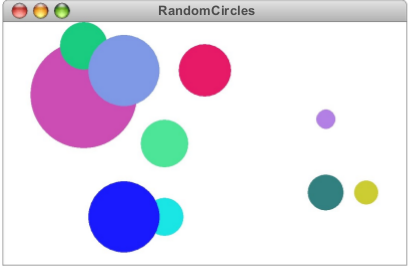
\includegraphics[width=4in]{random_circles.png}
\end{center}
The provided starter code contains examples of how to generate random numbers
and colors in the comments. It also contains several constants, which you should
use in your program as appropriate.
\subsection*{Challenge Problem -- Sorting an array}
In {\tt ArrayHelpers.java}, fill in the method {\tt sortArray}, which takes in
an array of integers and modifies it by rearranging its values so that the
integers are in sorted order, from smallest to largest.

There are many different ways to sort an array. For one idea of how to do this,
look at the Wikipedia page for ``bubble sort.''
\end{document}
